\scanpage{10}
% archive sheet number: 9
(4.3) est connu p\textsuperscript{\handwritten{\unsure{/}}}\unsure{\deleted{a}o|\deleted{o}a}\unsure{\deleted{r}u|\deleted{u}r|\deleted{n}u|\deleted{u}n}r tout $G$ par la seule connaissance de
\[
\mathrm{R}f_{\handwritten{!}}(A_X(d-d')\handwritten{[}2(d-d')\handwritten{]})\handwritten{\longrightarrow}A_Y.
\tag*{(4.4)}
\]
Ceci devrait bien donner la formule de projection au niveau des classes de cohomologie (qu'il faut bien entendu expliciter, soit ici, soit\inserted{(mieux)} à la fin du formulaire, en reprenant ce formulaire dans \deleted{\unsure{le ca}} le cas particulier \unsure{\deleted{d}r|\deleted{r}d}ecommand\unsure{\deleted{a}é|\deleted{é}a}\handwritten{,} parmi les variantes possibles).

\deleted{\unsure{b|a}}\handwritten{a}) \uline{Si} $d=d'$ \uline{et si} $\unsure{\deleted{g}f|\deleted{f}g}$ \uline{est quasi-fini} (et alors automatiquement plat, supposant que la dimension relative de $p$ est partout $d$), alors on retrouve l'homomorphisme trace de XVII ...

\deleted{\unsure{c|a|b}}\handwritten{b}) Si $f$ \uline{est lisse}, on retrouve l'\unsure{\deleted{g}h|\deleted{h}g|\deleted{j}h|\deleted{h}j}omomorphisme trace du par.2.

\deleted{\unsure{d|c}}\handwritten{c}) \uline{Transitivité} pour un composé $gf$ ($g:Y\handwritten{\longrightarrow}Z$, avec $Z$ lisse et compactifiable sur $S$).

\margin{\handwritten{d) ici}\begin{tikzpicture}[overlay,baseline]
\draw[gray,line width=.25pt] (0.18,0.15) .. controls (0.10,0.60) and (-0.02,0.70) .. (-0.45,0.66) .. controls (-0.92,0.64) and (-1.25,0.12) .. (-1.18,-0.10) .. controls (-1.10,-0.41) and (-0.45,-0.29) .. (0.18,0.15);
\draw[gray,line width=.25pt] (-.08,.60) -- (-.17,.56);
\draw[line width=.35pt] (0.10,0.15) -- (2.55,0.20);
\end{tikzpicture}}
\deleted{\unsure{e|d}}\handwritten{f}) Compatibilité avec \uline{Künneth}, quand on regarde $g_1\mathbin{\mathrm{x}}_S g_2:X_1\mathbin{\mathrm{x}}_S X_2\handwritten{\longrightarrow}Y_1\mathbin{\mathrm{x}}_S Y_2$. Compatibilité avec \uline{changement de base}\inserted{$S'\handwritten{\longrightarrow}S$.}

\deleted{\unsure{f}}\handwritten{e}) Compatibilité avec \uline{changement d'\unsure{\deleted{a}A|\deleted{A}a}nneau} $A\handwritten{\longrightarrow}A'$ (qui montr qu'il suffit de connaitre (4.4) pour les $A=(\underline{\mathrm{Z}}/n\underline{\mathrm{Z}})_S$ pour l'avoir pour tout $A$).

g) \uline{Indépendance par rapport à} $S$ (si on se donne $S\handwritten{\longrightarrow}\deleted{\unsure{S|et|S'|St}}T$ lisse, de sorte que l'on peut regarder $X$ et $Y$ comme étant sur $T$ ...).

h) \uline{Formule d'échange}, relatif au cas où on a un diagramme cartésien
\diagram{\begin{tikzcd}[ampersand replacement=\&,row sep=2em,column sep=2em,execute at end picture={
\draw[gray,line width=.25pt] ([xshift=-1pt,yshift=13pt]xx.north west)
.. controls ([xshift=-22pt,yshift=19pt]xx.north west) and ([xshift=-22pt,yshift=-4pt]xx.west) .. ([xshift=-10pt,yshift=-7pt]yy.south west)
.. controls ([xshift=-3pt,yshift=-19pt]yy.south) and ([xshift=11pt,yshift=-18pt]yyp.south) .. ([xshift=16pt,yshift=-2pt]yyp.east)
.. controls ([xshift=20pt,yshift=13pt]yyp.east) and ([xshift=16pt,yshift=11pt]yyp.north east) .. ([xshift=4pt,yshift=9pt]yyp.north west)
.. controls ([xshift=-8pt,yshift=13pt]yyp.north west) and ([xshift=21pt,yshift=-21pt]xx.east) .. ([xshift=15pt,yshift=-13pt]xx.east)
.. controls ([xshift=10pt,yshift=3pt]xx.east) and ([xshift=3pt,yshift=7pt]xx.north) .. ([xshift=-1pt,yshift=3pt]xx.north west);
}]
|[alias=xx]| X \handwritten{\arrow[d,"f"{left},line width=.8pt]} \& X' \handwritten{\arrow[l,"h"{above},line width=.8pt]} \handwritten{\arrow[d,"f'"{right},line width=.55pt]} \\
|[alias=yy]| Y \& |[alias=yyp]| Y' \handwritten{\arrow[l,"g"{above},line width=.8pt]}
\end{tikzcd}}
de schémas sur $S$: appl\unsure{\deleted{j}i|\deleted{i}j}quant $g^*$ à $\mathrm{Tr}_f$, et appliquant \deleted{\unsure{la for}} l'isomorphisme de changement de base pour $\mathrm{R}f_{\handwritten{!}}$ et $g^*$, on doit trouver $\mathrm{Tr}_{f'}$. On supposera bien sûr $Y$ et $Y'$ lisses sur $S$, $X$ plat sur $S$, et pour que $X'$ soit plat sur $S$, il faut évidemment une hypothèse genre Tor-indépendance de $X$ et $Y'$ sur $Y$. Cela doit marcher en tous cas si $X$ est également lisse sur $S$, et si $f$ et $g$ sont \uline{transversaux} (EGA IV \unsure{\deleted{2}1|\deleted{1}2|\deleted{7}1|\deleted{1}7}7...).
